\section*{B.5 Fallbeispiele Mechatronik}

\subsection{Stellen Sie Defition und Motivation f\"ur Mechatronik im Automobilbau dar. Welche Aufgabenstellungen ergeben sich durch Mechatronik im r\"aumlichen Sinn? (S.125)}
Mechatronik = Mechanik + Elektronik
\begin{itemize}
\item Integration aufgrund Platzmangel / zur Gewichtssenkung
\item modulare, testbare Einheiten $\rightarrow$ Produktions- und Testprozess vereinfacht
\item Einfache Variantenbildung durch Gleichteilproduktion und anschließende Band-Ende Programmierung
\item Qualitätssteigerung und Kostensenkung durch Minimierung der elektrischen und mechanischen Kontaktierung
\item Kostensenkung durch Entfeinerung der Komponenten und anschließenden Toleranzabgleich im Rahmen der 
Band-Ende Programmierung
\item Verbessertes EMV-Verhalten durch kürzere elektrische Verbindungen
\end{itemize}
Aufgabenstellungen: hohe Temperaturen (zB: Motor, Getriebe), hohe mechanische Belastung (Vibration), hohe 
chemische Belastung (zB: Getriebeöl)

\subsection{Was charakterisiert ein modernes Motorkühlungssystem und welche Vorteile ergeben sich dadurch?}
In modernen Motorkühlungssystem sind Kühlwasser- und Luftfluss von
einander getrennt (Luftkreislauf nur mehr elektrisch, Wasserkreislauf
immer öfter elektrisch). Die Kühlung wird auf den aktuellen Bedarf
geregelt und nicht auf die Drehzahl des Motors (RPM $\neq$ Motorleistung).\\
Vorteile:
\begin{itemize}
\item Verhindert/Reduziert Heizabstellverlust(hot soak)
\item Geringerer Kraftstoffverbrauch durch Entkoppelung von der
  Kurbelwelle. Motortemperatur wird optimiert $\rightarrow$ senkt Kraftstoffverbrauch.
\item Schnelleres erreichen der Betriebstemperatur(Motor, Katalysator)
  $\rightarrow$ Bessere Emmisionswerte beim Start.
\item Ermöglicht Modularisierung und vereinfacht das Packaging.
\end{itemize}

\subsection{Welche elektrischen und elektronischen Komponenten
  befinden sich in einem modernen Klimager\"at und welche Hauptaufgabe
  haben sie.}
In der Klimaanlage wird ein Kühlmittel (hier $CO_2$) verwendet. 
\begin{center}
  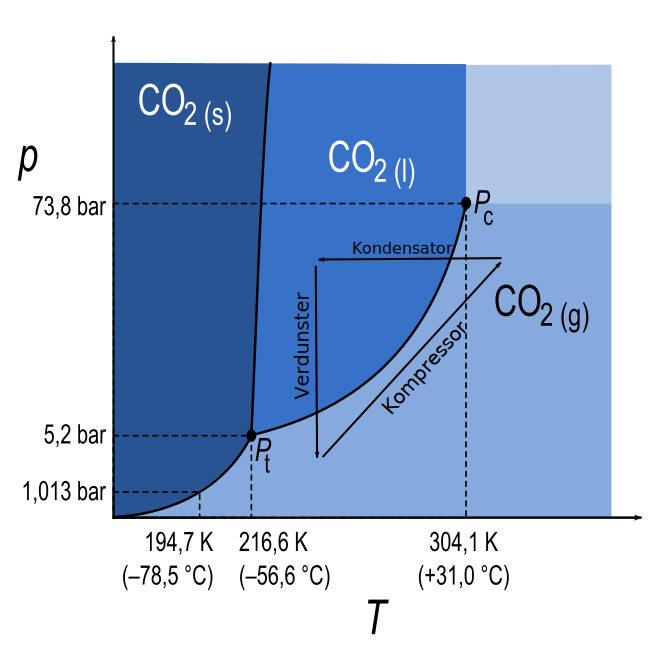
\includegraphics[width=0.7\textwidth]{pics/Carbon_dioxide_p-T_phase_diagram}
\end{center}

\begin{description}
\item[Kompressor:] Komprimiert das Kühlmittel $\rightarrow$ Erwärmt sich
\item[Kondensator:] Das Kühlmittel wird durch die Außenluft abgekühlt
  und kondensiert.
\item[Verdampfer:] Das Kühlmittel wird durch eine Düse in den
  Verdampfer eingesprüht und verdampft wegen des geringeren
  Drucks. $\rightarrow$ Kühlmittel veringert die Temperatur. Die
  Außenluft durchströmt den Verdampfer und kühlt ab (\textgreater
  0\textdegree C um eisbildung zu vermeiden). Der Wirkungsgrad ist
  proportional zur Luftfäuchtigkeit.
\item[Heizkörper/elektrischer Zuheizer:] Die vom Verdampfer kommende
  Luft wird über die Heizung geführt. Dabei wird das
  Motorkühlungswasser als Wärmequelle verwendet. Bei Diesel-Motoren
  ist häufig eine elektrische Zuheizung notwendig da vor allem nach
  dem Start keine ausreichende Wärmeleistung vom Motor zur verfügung steht. 
\item[Gebläse:] Das Gebläse fördert die gewünschte Luftmenge und wird
  abhängig von der Geschwindigkeit reguliert.
\item[Filter:] Filtert die Außenluft.
\item[Bediengerät:] Benuzereinstellungen \dots
\end{description}


\subsection{Skizzieren und beschreiben Sie die elektrische Architektur eines modernen Klimager\"ats.}
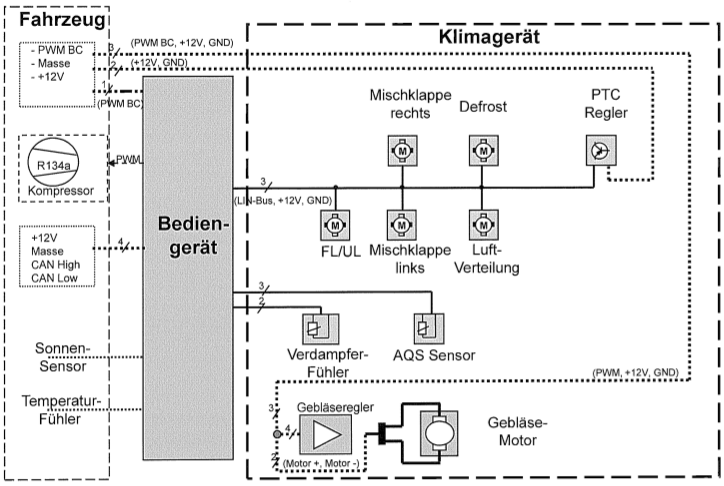
\includegraphics[width=\textwidth]{pics/architekturKlimaanlage}
